\section{Unità di Controllo microprogrammata}

\begin{figure}[H]
      \centering
      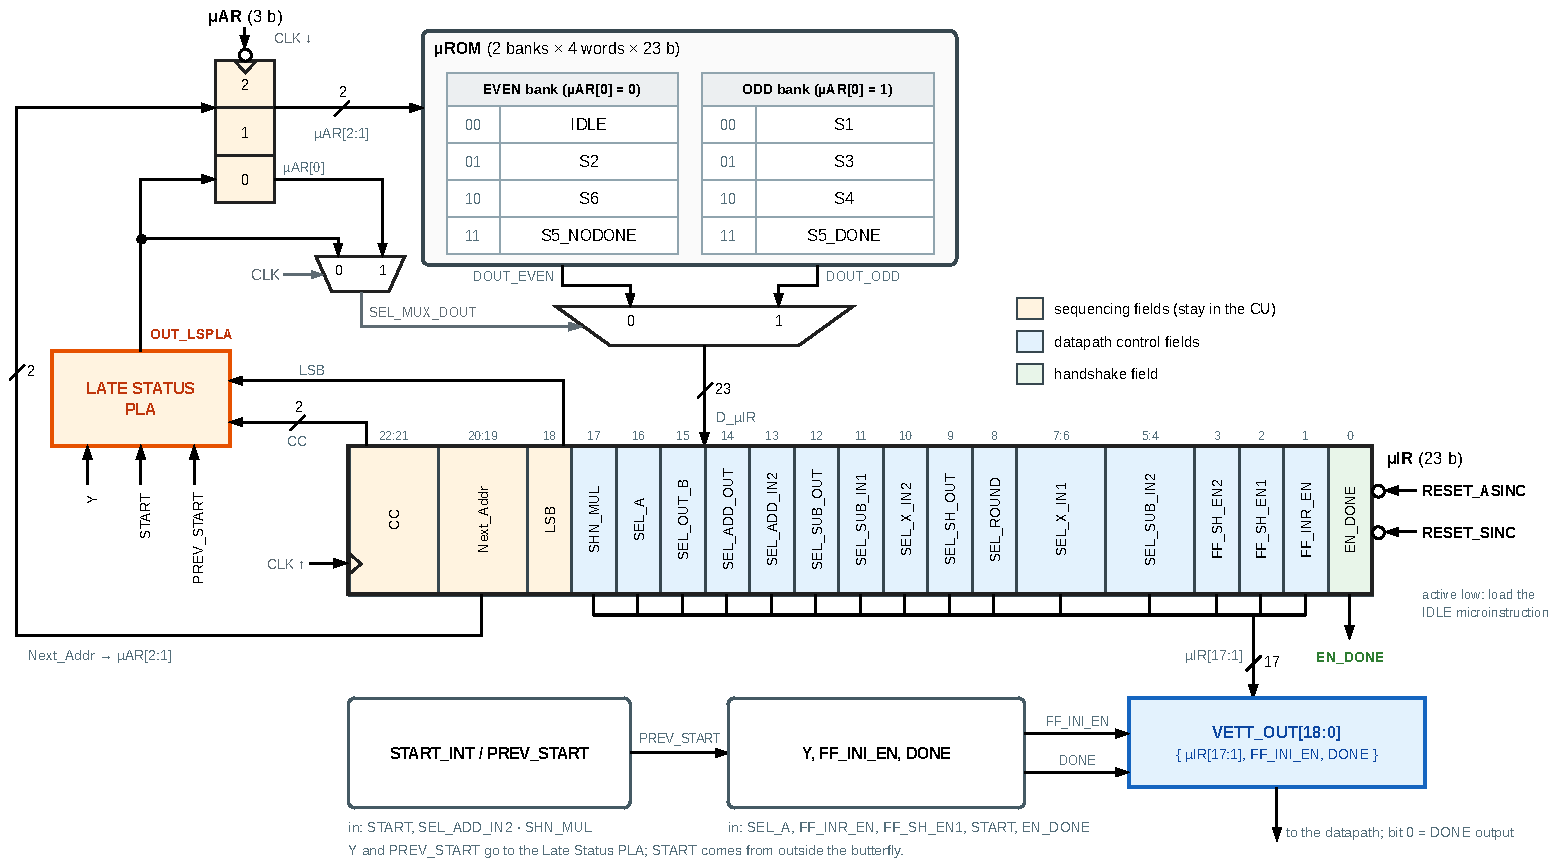
\includegraphics[width=1\textwidth]{fig08_cu_microprogrammed}
      \caption{Schema della CU microprogrammata}
      \label{fig:CU_uProg_schema}
\end{figure} 

\noindent Il diagramma degli stati presentato nella precedente sezione è stato descritto in VHDL attraverso una Unità di Controllo microprogrammata, in cui si è utilizzata la tecnica del LATE STATUS. L'architettura è costituita da quattro elementi fondamentali: la $\mu ROM$, il registro dei micro-indirizzi $\mu AR$, il registro in cui vengono salvate le $\mu$Istruzioni $\mu IR$ ed il blocco logico di selezione.

\noindent Il registro $\mu AR$, il quale si è scelto che campioni sul fronte di discesa del clock, memorizza la codifica dello stato (e quindi il $\mu$indirizzo) corrente. In particolare, il $\mu AR$ ha un parallelismo di 3 bit, poiché la codifica degli stati avviene su soli 3 bit, dato che nello State Diagram sono presenti 8 stati distinti.

\noindent La micromemoria, caratterizzata da un indirizzo su due bit, è divisa in due banchi da 4 locazioni ciascuna: quello delle righe pari, che racchiude le microistruzioni relative agli indirizzi con LSB=0 e quello delle righe dispari (relative agli indirizzi per cui LSB=1). Ogni parola contiene una microistruzione da 23 bit. 

\noindent Invece, il registro $\mu IR$, caratterizzato dal medesimo parallelismo delle parole della $\mu ROM$, campiona sul fronte di salita del segnale di sincronizzazione la $\mu$Istruzione selezionata.

\noindent Infine, la logica di Selezione, formata dalla Late Status PLA e da due multiplexer, decide se verrà eseguita l'istruzione associata all'indirizzo pari o a quello dispari. Infatti, quando il $\mu AR$ punta ad una riga della memoria, vengono lette contemporaneamente entrambe le microistruzioni possibili dai due banchi. La parola voluta viene selezionata da un multiplexer, che ha come selettore l'uscita della PLA, che coincide con il LSB della codifica del prossimo stato. In particolare, tale bit viene anche salvato, in corrispondenza del falling edge del clock, nel bit meno significativo del $\mu$AR. Per questo si è implementato un secondo multiplexer, pilotato dal clock stesso, che sceglie da dove prendere il selettore della prossima $\mu$Istruzione SEL\_MUX\_DOUT. Quando il clock è basso, ossia dopo il fronte di discesa e fino al fronte di salita successivo, il multiplexer secondario instrada direttamente l'uscita della Late Status PLA (OUT\_LSPLA): in questo modo, sul fronte di salita, il $\mu IR$ campiona la $\mu$Istruzione scelta con il valore più aggiornato dei segnali di stato. Invece, quando il clock è alto (dal fronte di salita fino al fronte di discesa successivo), il multiplexer secondario è girato sull'ingresso opposto e instrada il bit meno significativo salvato nel $\mu$AR.

\noindent Al fine di gestire in maniera più pulita la definizione della entity della CU e i port map di tale component, si sono raggruppate tutte le uscite dell'unità di controllo in un unico vettore VETT\_OUT, la cui mappatura con segnali significativi è presentata nella tabella a seguire.

\begin{comment}
\begin{figure}[H]
      \centering
      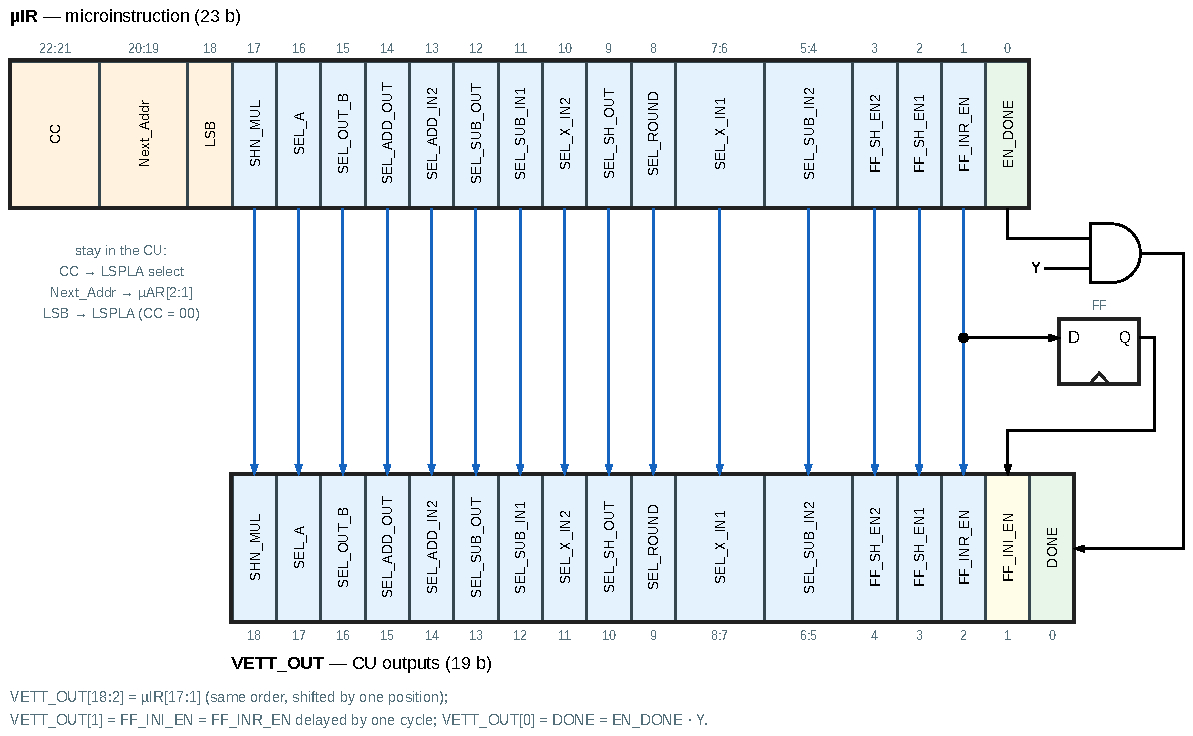
\includegraphics[width=0.9\textwidth]{fig13_microword_vett_out}
      \caption{Tabella che associa, a ciascun bit di VETT\_OUT, il segnale di controllo del datapath }
\end{figure}
\end{comment}

\begin{table}[H]
\centering
\begin{tabular}{|c|l|}
\hline
\textbf{Indice} & \textbf{Nome Segnale} \\ \hline
18 & \texttt{SHN\_MUL} \\ \hline
17 & \texttt{SEL\_A} \\ \hline
16 & \texttt{SEL\_OUT\_B} \\ \hline
15 & \texttt{SEL\_ADD\_OUT} \\ \hline
14 & \texttt{SEL\_ADD\_IN2} \\ \hline
13 & \texttt{SEL\_SUB\_OUT} \\ \hline
12 & \texttt{SEL\_SUB\_IN1} \\ \hline
11 & \texttt{SEL\_X\_IN2} \\ \hline
10 & \texttt{SEL\_SH\_OUT} \\ \hline
9  & \texttt{SEL\_ROUND} \\ \hline
8  & \texttt{SEL\_X\_IN1(1)} \\ \hline
7  & \texttt{SEL\_X\_IN1(0)} \\ \hline
6  & \texttt{SEL\_SUB\_IN2(1)} \\ \hline
5  & \texttt{SEL\_SUB\_IN2(0)} \\ \hline
4  & \texttt{FF\_SH\_EN2} \\ \hline
3  & \texttt{FF\_SH\_EN1} \\ \hline
2  & \texttt{FF\_INR\_EN} \\ \hline
1  & \texttt{FF\_INI\_EN} \\ \hline
0  & \texttt{DONE} \\ \hline
\end{tabular}
\caption{Tabella che associa, a ciascun bit di VETT\_OUT, il segnale di Done o un segnale di controllo da inviare al datapath}
\end{table}

\noindent In conclusione, si evidenzia che il blocco "Y, FF\_INI\_EN, DONE" presente in Figura \ref{fig:CU_uProg_schema}, è composto dalle logiche presentate nella sottosezione \ref{subsec:Y,PREV_START,DONE} per la gestione dei tre segnali indicati.


\subsection{La micromemoria $\mu ROM$}

\begin{comment}
\begin{figure}[H]
      \centering
      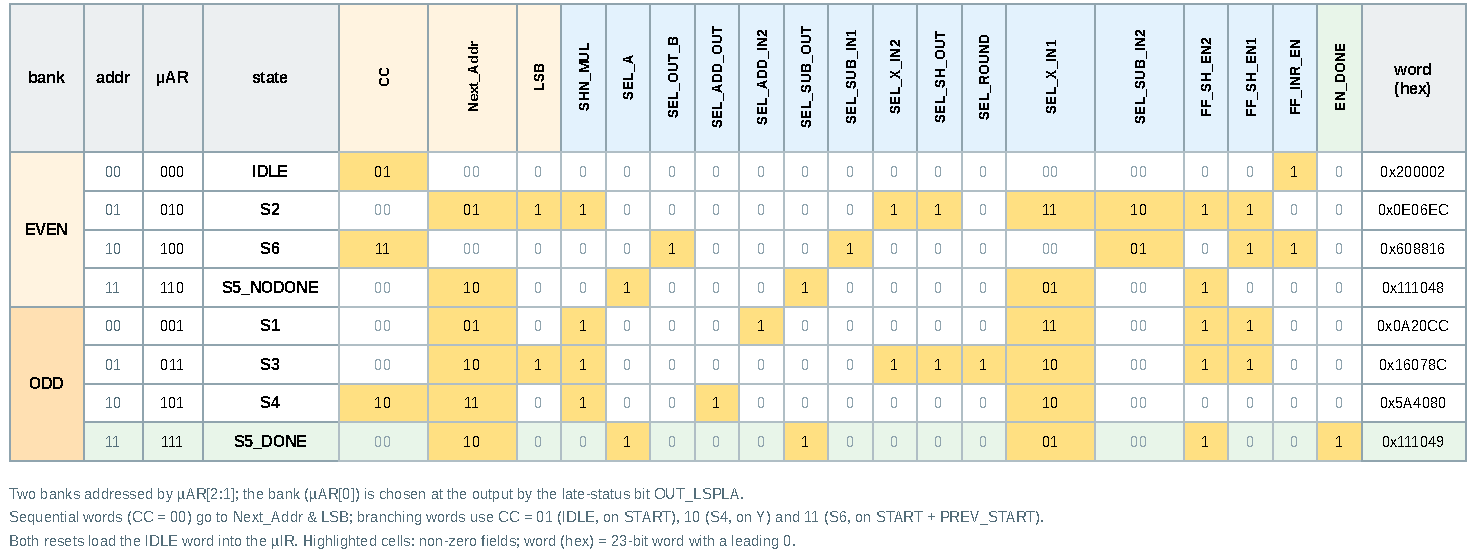
\includegraphics[width=1\textwidth]{fig14_urom_contents}
      \caption{$\mu ROM$}
\end{figure}

\end{comment}
\begin{comment}



\end{comment}

\noindent Come precedentemente detto, la $\mu ROM$ implementata presenta due diversi banchi di memoria: uno per le locazioni pari, e uno per gli indirizzi dispari. Poiché, come evidente dal diagramma degli stati, si hanno in totale $2^3  =  8$ stati, la loro codifica avviene su 3 bit e ciascun banco della micromemoria ha 4 locazioni; l'indirizzo, invece, è su 2 bit e risulta in comune ai due banchi.

\noindent Ogni parola, che codifica una $\mu$Istruzione della macchina, contiene 23 bit; i primi tre campi (CC, Next\_Addr e LSB) gestiscono la logica di sequenziamento, mentre gli altri rappresentano i segnali di controllo. La seguente tabella mostra la codifica di ciascuna $\mu$Istruzione, per ogni stato della macchina. In particolare, escludendo la prima riga in cui è indicata la codifica dello stato in analisi, nelle righe successive sono indicate le codifiche in binario dei vari segnali. Concatenandoli verticalmente, dall'alto verso il basso, è possibile ottenere il contenuto della parola associata allo specifico stato e presente nella $\mu ROM$ (dall' MSB all' LSB).


\begin{table}[H]
\centering


\setlength{\tabcolsep}{4pt} % Spazio orizzontale tra le colonne
\renewcommand{\arraystretch}{1.2} % Spazio verticale tra 
\begin{tabular}{|l|c|c|c|c|c|c|c|c|}
\hline
\textbf{Segnale} & \textbf{IDLE} & \textbf{ST.1} & \textbf{ST.2} & \textbf{ST.3} & \textbf{ST.4} & \textbf{ST.5\_DONE} & \textbf{ST.5\_NODONE} & \textbf{ST.6} \\ \hline
Codifica Stato & 000 & 001 & 010 & 011 & 101 & 111 & 110 & 100 \\ \hline
CC & 01 & 00 & 00 & 00 & 10 & 00 & 00 & 11 \\ \hline
Next\_Addr & 00 & 01 & 01 & 10 & 11 & 10 & 10 & 00 \\ \hline
LSB & 0 & 0 & 1 & 1 & 0 & 0 & 0 & 0 \\ \hline
SHN\_MUL & 0 & 1 & 1 & 1 & 1 & 0 & 0 & 0 \\ \hline
SEL\_A & 0 & 0 & 0 & 0 & 0 & 1 & 1 & 0 \\ \hline
SEL\_OUT\_B & 0 & 0 & 0 & 0 & 0 & 0 & 0 & 1 \\ \hline
SEL\_ADD\_OUT & 0 & 0 & 0 & 0 & 1 & 0 & 0 & 0 \\ \hline
SEL\_ADD\_IN2 & 0 & 1 & 0 & 0 & 0 & 0 & 0 & 0 \\ \hline
SEL\_SUB\_OUT & 0 & 0 & 0 & 0 & 0 & 1 & 1 & 0 \\ \hline
SEL\_SUB\_IN1 & 0 & 0 & 0 & 0 & 0 & 0 & 0 & 1 \\ \hline
SEL\_X\_IN2 & 0 & 0 & 1 & 1 & 0 & 0 & 0 & 0 \\ \hline
SEL\_SH\_OUT & 0 &0  & 1 & 1 & 0 & 0 & 0 &0 \\ \hline
SEL\_ROUND & 0 & 0 & 0 & 1 & 0 & 0 & 0 & 0 \\ \hline
SEL\_X\_IN1 & 00 & 11 & 11 & 10 & 10 & 01 &01 & 00 \\ \hline
SEL\_SUB\_IN2 & 00 & 00 & 10 & 00 & 00 & 00 & 00 & 01 \\ \hline
FF\_SH\_EN2& 0 & 1 & 1 & 1 & 0 & 1 & 1& 0  \\ \hline
FF\_SH\_EN1 & 0 & 1 & 1 & 1 & 0 & 0 & 0 & 1 \\ \hline
FF\_INR\_EN & 1 & 0 & 0 & 0 & 0 & 0 & 0 & 1 \\ \hline
EN\_DONE & 0 & 0 & 0 & 0 & 0 & 1 & 0 & 0 \\ \hline
\end{tabular}%
%} % chiusura resizebox
\caption{Contenuto di ciascuna $\mu$Istruzione e codifica degli stati della macchina}
\end{table}

\noindent In conclusione, il contenuto della $\mu ROM$ è riportato in modo compatto nella tabella sottostante:

\begin{table}[H]
    \centering
    \begin{tabular}{|c|c|c|}
        \hline
        \textbf{Nome dello stato} & \textbf{Indirizzo associato} & \textbf{Contenuto Locazione} \\
        \hline
        IDLE & 000 & 01000000000000000000010 \\
        \hline
        STATO 1 & 001 & 00010100010000011001100 \\
        \hline
        STATO 2 &  010 & 00011100000011011101100 \\
        \hline
        STATO 3 & 011 & 00101100000011110001100 \\
        \hline
        STATO 4 & 101 & 10110100100000010000000 \\
        \hline
        STATO 5\_DONE & 111 & 00100010001000001001001 \\
        \hline
        STATO 5\_NODONE & 110 & 00100010001000001001000 \\
        \hline
        STATO 6 & 100 & 11000001000100000010110 \\
        \hline
    \end{tabular}
    \caption{Contenuto della $\mu ROM$}
    \label{tab:stati_indirizzi}
\end{table}

\subsection{Late Status PLA}
\noindent Tale rete combinatoria gestisce, come già spiegato, la logica dei salti. Come input, presenta ingressi di stato START, $PREV\_START$, $Y$ ed LSB, ovvero il bit meno significativo associato alla codifica dell'istruzione successiva, nel caso in cui non sia necessario saltare. Il campo CC, il 'Condition Code', è codificato su 2 bit, poiché nel pallogramma sono presenti solo 3 diversi salti a 2 vie, ed esso serve alla Late Status PLA per discriminare di quali segnali tenere conto per generare l'uscita $OUT\_LSPLA$. Tale uscita, nell'architettura progettata, è il LSB della codifica dello stato a cui transire, il quale verrà salvato nella locazione 0 del $\mu AR$ in corrispondenza del fronte di discesa del clock del sistema.

\noindent Si è deciso che il campo CC sia pari a 01 quando nel $\mu IR$ è salvata la riga dei comandi associata allo stato di IDLE; in tal caso, in accordo con lo State Diagram e la codifica degli stati scelta, il segnale di START è il responsabile della scelta. Invece, per lo stato 4, CC  = 10 e l'output della PLA coincide con Y, il cui valore andrà a determinare se verrà compiuto il salto in STATO 5\_DONE o in STATO 5\_NODONE. Di contro, nello STATO 6 (CC = 11) intervengono i segnali $START$ e $PREV\_START$ per decidere se tornare in IDLE o meno. Infine, in tutti gli altri stati il condition code vale 00; in tali stati non sono previsti salti e, di conseguenza, il banco della $\mu ROM$ da selezionare dipende unicamente dal campo $LSB$ salvato nel $\mu IR$ ($OUT\_LSPLA \quad = \quad LSB$).

\noindent Si riporta di seguito il semplice multiplexer che descrive lo schematico della PLA progettata.

\begin{figure}[H]
      \centering
      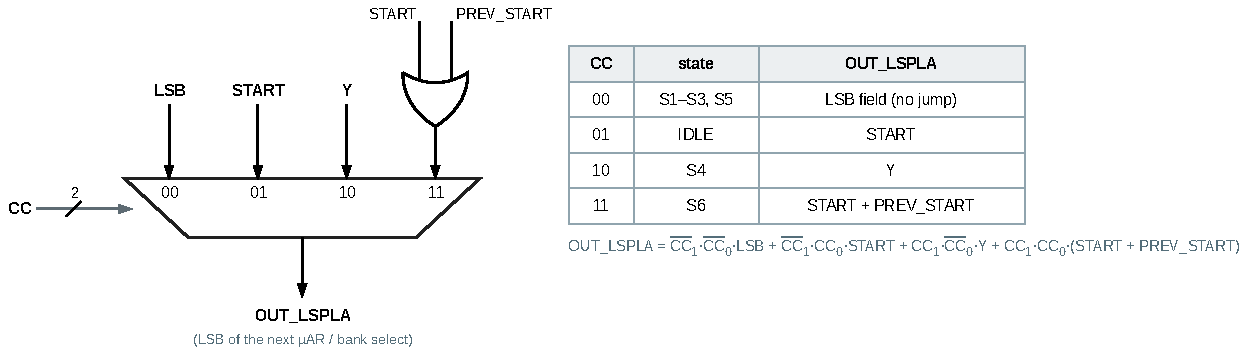
\includegraphics[width=1\textwidth]{fig09_late_status_pla}
      \caption{Schematico del blocco Late Status PLA}
\end{figure}

\noindent Si riportano, per completezza ed a titolo d'esempio, due transizioni logiche del sistema. Per ipotesi, si parte dallo stato di IDLE, con codifica "000". Il campo Next\_Addr vale "00". Dopo che questi due bit vengono salvati nelle prime due locazioni del $\mu AR$, la $\mu ROM$ legge due possibili future righe: quella relativa allo STATO 1 (indirizzo dispari "00(1)") e quella relativa allo IDLE (indirizzo pari "00(0)"). Poiché CC è impostato a "01" in IDLE, la PLA selezionerà il banco pari o dispari a seconda che lo start risulti attivo o meno; la riga scelta verrà salvata nel $\mu IR$ in corrispondenza del fronte di salita seguente del clock.
\noindent Si supponga, invece, che la macchina sia nello STATO 4, per il quale Next\_Addr vale "11". La $\mu ROM$ legge i due possibili percorsi: STATO 5\_DONE (indirizzo dispari "11(1)") o STATO 5\_NODONE (indirizzo pari "11(0)"). La PLA valuta la condizione Y e forzerà OUT\_LSPLA per la selezione dello stato futuro a '0' od a '1'.


\subsection{Reset della Butterfly}
\label{subsec:reset}
La macchina di controllo progettata per la Butterfly, come visibile nella parte destra della Figura \ref{fig:CU_uProg_schema}, presenta due tipologie di reset attivi bassi: uno sincrono e uno asincrono. Quando uno di questi si attiva (quello sincrono deve essere attivo attorno al rising edge del clock), la macchina viene riportata nello stato di IDLE, poiché l'uscita del $\mu IR$ viene impostata pari alla parola della $\mu ROM$ associata allo stato di attesa ("01000000000000000000010").

\noindent In particolare, il reset asincrono è stato introdotto al fine di poter resettare la macchina al power-on, fase in cui il clock potrebbe essere instabile. Questo segnale deve essere utilizzato solo in tale istanza. Invece, il reset sincrono è da utilizzare quando il clock del sistema risulta stabile. Si specifica che, in entrambi i casi, se la macchina viene interrotta mediante uno di questi 2 segnali prima che vengano prodotti i risultati di un'elaborazione, non si osserveranno i corretti dati in uscita negli intervalli temporali in cui sono attesi.

\noindent In conclusione, si indica che la scelta di impostare un valore nel $\mu IR$ rispetto all'azzeramento del $\mu AR$ è dovuta al fatto che, in tale modo, si riesce a essere più reattivi a un futuro segnale di start; infatti, dopo un breve ritardo, la Late Status PLA riceve già i vari bit di controllo associati allo stato di IDLE, al fine di poter generare correttamente il LSB dello stato futuro. Di contro, applicando i reset sul $\mu AR$, sarebbe necessario attendere il fronte di salita successivo al momento in cui il registro viene azzerato, per fornire alla PLA il Condition Code relativo all'IDLE.
